%!TEX TS-program = xelatex

% Шаблон документа LaTeX создан в 2018 году
% Алексеем Подчезерцевым
% В качестве исходных использованы шаблоны
% 	Данилом Фёдоровых (danil@fedorovykh.ru) 
%		https://www.writelatex.com/coursera/latex/5.2.2
%	LaTeX-шаблон для русской кандидатской диссертации и её автореферата.
%		https://github.com/AndreyAkinshin/Russian-Phd-LaTeX-Dissertation-Template

\documentclass[a4paper,14pt]{article}


%%% Работа с русским языком
\usepackage[english,russian]{babel}   %% загружает пакет многоязыковой вёрстки
\usepackage{fontspec}      %% подготавливает загрузку шрифтов Open Type, True Type и др.
\defaultfontfeatures{Ligatures={TeX},Renderer=Basic}  %% свойства шрифтов по умолчанию
\setmainfont[Ligatures={TeX,Historic}]{Times New Roman} %% задаёт основной шрифт документа
\setsansfont{Comic Sans MS}                    %% задаёт шрифт без засечек
\setmonofont{Courier New}
\usepackage{indentfirst}
\frenchspacing

\renewcommand{\epsilon}{\ensuremath{\varepsilon}}
\renewcommand{\phi}{\ensuremath{\varphi}}
\renewcommand{\kappa}{\ensuremath{\varkappa}}
\renewcommand{\le}{\ensuremath{\leqslant}}
\renewcommand{\leq}{\ensuremath{\leqslant}}
\renewcommand{\ge}{\ensuremath{\geqslant}}
\renewcommand{\geq}{\ensuremath{\geqslant}}
\renewcommand{\emptyset}{\varnothing}

%%% Дополнительная работа с математикой
\usepackage{amsmath,amsfonts,amssymb,amsthm,mathtools} % AMS
\usepackage{icomma} % "Умная" запятая: $0,2$ --- число, $0, 2$ --- перечисление

%% Номера формул
%\mathtoolsset{showonlyrefs=true} % Показывать номера только у тех формул, на которые есть \eqref{} в тексте.
%\usepackage{leqno} % Нумерация формул слева	

%% Перенос знаков в формулах (по Львовскому)
\newcommand*{\hm}[1]{#1\nobreak\discretionary{}
	{\hbox{$\mathsurround=0pt #1$}}{}}

%%% Работа с картинками
\usepackage{graphicx}  % Для вставки рисунков
\graphicspath{{images/}}  % папки с картинками
\setlength\fboxsep{3pt} % Отступ рамки \fbox{} от рисунка
\setlength\fboxrule{1pt} % Толщина линий рамки \fbox{}
\usepackage{wrapfig} % Обтекание рисунков текстом

%%% Работа с таблицами
\usepackage{array,tabularx,tabulary,booktabs} % Дополнительная работа с таблицами
\usepackage{longtable}  % Длинные таблицы
\usepackage{multirow} % Слияние строк в таблице
\usepackage{float}% http://ctan.org/pkg/float

%%% Программирование
\usepackage{etoolbox} % логические операторы


%%% Страница
\usepackage{extsizes} % Возможность сделать 14-й шрифт
\usepackage{geometry} % Простой способ задавать поля
\geometry{top=20mm}
\geometry{bottom=20mm}
\geometry{left=20mm}
\geometry{right=10mm}
%
%\usepackage{fancyhdr} % Колонтитулы
% 	\pagestyle{fancy}
%\renewcommand{\headrulewidth}{0pt}  % Толщина линейки, отчеркивающей верхний колонтитул
% 	\lfoot{Нижний левый}
% 	\rfoot{Нижний правый}
% 	\rhead{Верхний правый}
% 	\chead{Верхний в центре}
% 	\lhead{Верхний левый}
%	\cfoot{Нижний в центре} % По умолчанию здесь номер страницы

\usepackage{setspace} % Интерлиньяж
\onehalfspacing % Интерлиньяж 1.5
%\doublespacing % Интерлиньяж 2
%\singlespacing % Интерлиньяж 1

\usepackage{lastpage} % Узнать, сколько всего страниц в документе.

\usepackage{soul} % Модификаторы начертания

\usepackage{hyperref}
\usepackage[usenames,dvipsnames,svgnames,table,rgb]{xcolor}
\hypersetup{				% Гиперссылки
	unicode=true,           % русские буквы в раздела PDF
	pdftitle={Заголовок},   % Заголовок
	pdfauthor={Автор},      % Автор
	pdfsubject={Тема},      % Тема
	pdfcreator={Создатель}, % Создатель
	pdfproducer={Производитель}, % Производитель
	pdfkeywords={keyword1} {key2} {key3}, % Ключевые слова
	colorlinks=true,       	% false: ссылки в рамках; true: цветные ссылки
	linkcolor=black,          % внутренние ссылки
	citecolor=black,        % на библиографию
	filecolor=magenta,      % на файлы
	urlcolor=black           % на URL
}
\makeatletter 
\def\@biblabel#1{#1. } 
\makeatother
\usepackage{cite} % Работа с библиографией
%\usepackage[superscript]{cite} % Ссылки в верхних индексах
%\usepackage[nocompress]{cite} % 
\usepackage{csquotes} % Еще инструменты для ссылок

\usepackage{multicol} % Несколько колонок

\usepackage{tikz} % Работа с графикой
\usepackage{pgfplots}
\usepackage{pgfplotstable}

% ГОСТ заголовки
\usepackage[font=small]{caption}
%\captionsetup[table]{justification=centering, labelsep = newline} % Таблицы по правобу краю
%\captionsetup[figure]{justification=centering} % Картинки по центру


\newcommand{\tablecaption}[1]{\addtocounter{table}{1}\small \begin{flushright}\tablename \ \thetable\end{flushright}%	
\begin{center}#1\end{center}}

\newcommand{\imref}[1]{рис.~\ref{#1}}

\usepackage{multirow}
\usepackage{spreadtab}
\newcolumntype{K}[1]{@{}>{\centering\arraybackslash}p{#1cm}@{}}


\usepackage{xparse}
\usepackage{fancyvrb}

\RecustomVerbatimCommand{\VerbatimInput}{VerbatimInput}
{
	fontsize=\footnotesize    
}

\usepackage{tocloft}
\renewcommand{\cftsecleader}{\cftdotfill{\cftdotsep}}
\begin{document} % конец преамбулы, начало документа
	\begin{titlepage}
	\begin{center}
 		ФЕДЕРАЛЬНОЕ  ГОСУДАРСТВЕННОЕ АВТОНОМНОЕ \\
		ОБРАЗОВАТЕЛЬНОЕ УЧРЕЖДЕНИЕ ВЫСШЕГО ОБРАЗОВАНИЯ\\
		«НАЦИОНАЛЬНЫЙ ИССЛЕДОВАТЕЛЬСКИЙ УНИВЕРСИТЕТ\\
		«ВЫСШАЯ ШКОЛА ЭКОНОМИКИ»
	\end{center}
	
	\begin{center}
		\textbf{Московский институт электроники и математики}
		
		\textbf{им. А.Н.Тихонова НИУ ВШЭ}
		
		\vspace{2ex}
		
		\textbf{Департамент компьютерной инженерии}
	\end{center}
	\vspace{1ex}	
	
	\begin{center}
	\textbf{ОТЧЕТ\\
		ПО ЛАБОРАТОРНОЙ РАБОТЕ №6
	}
	\end{center}	
	\vspace{2ex}
	\begin{center}
		по дисциплине «Проектирование систем на кристалле»
	\end{center}	

	\vspace{2ex}

	\begin{flushright}
		\textbf{Выполнили:}
		
		\vspace{2ex}
		
		Студенты группы БИВ174
		
		Бригада №5
		
		\vspace{2ex}
		
		Подчезерцев Алексей Евгеньевич
		
		Солодянкин Андрей Александрович
		\vspace{2ex}
		
	\end{flushright}

	\vfill
	\begin{center}
		Москва \the\year \, г.
	\end{center}
	
\end{titlepage}
\addtocounter{page}{1}
	\tableofcontents
	\pagebreak
	\section{Задание}
	
	\begin{enumerate}
		\item Реализуйте однотактный и многотактный модули в поведенческом стиле.
		
		\item Реализуйте данный модуль с параметром, равным з начению 5, проанализируйте его	характеристики и убедитесь, что они не изменились по сравнению с предыдущими	реализациями. Убедитесь в работоспособности получившихся реализаций, выполните имплементацию и сравните их	характеристики с характеристиками исходной реализации.
	
		\item Выполните имплементацию модуля со значением параметра n = 5, проанализируйте его	характеристики и убедитесь, что они не изменились. Убедитесь в работоспособности получившихся реализаций, выполните имплементацию и сравните их
		характеристики с характеристиками исходной реализации.
		 
	\end{enumerate}
	
	\section{Дополнительные задания}
	
	\subsection{Задание 1}
	
	Реализуйте однотактный и многотактный модули в поведенческом стиле.
	
	На рис. \ref{fig:z103} представлен результат компиляции однотактного модуля в поведенческом стиле, на рис. \ref{fig:z106} многотактного модуля.
	
		\begin{figure}[H]
			\centering
			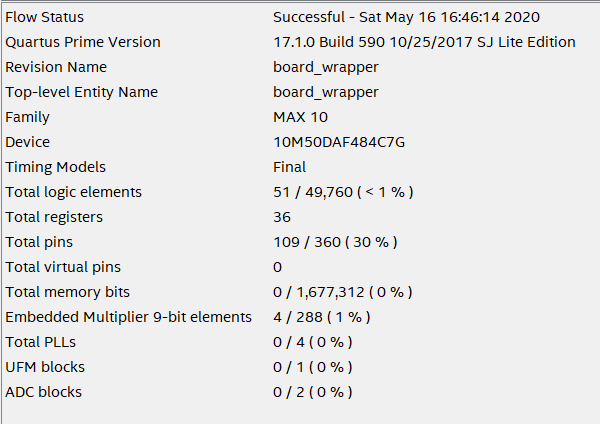
\includegraphics[width=0.8\linewidth]{images/z1_03}
			\caption{Результат компиляции однотактного модуля}
			\label{fig:z103}
		\end{figure}
			
		\begin{figure}[H]
			\centering
			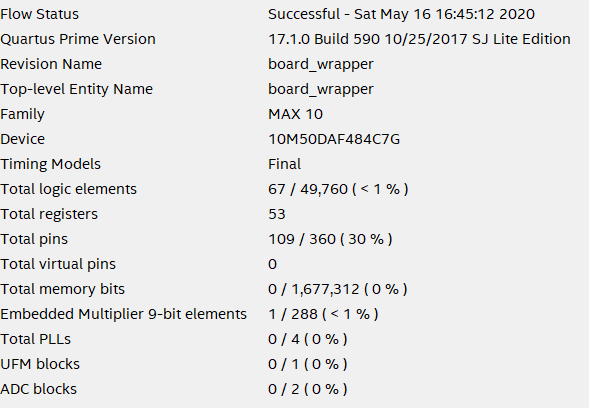
\includegraphics[width=0.8\linewidth]{images/z1_06}
			\caption{Результат компиляции многотактного модуля}
			\label{fig:z106}
		\end{figure}
		
	
	\subsection{Задание 2}
	
	Реализуйте данный модуль с параметром, равным значению 5, проанализируйте его характеристики и убедитесь, что они не изменились по сравнению с предыдущими	реализациями. Убедитесь в работоспособности получившихся реализаций, выполните имплементацию и сравните их характеристики с характеристиками исходной реализации.
	
	\begin{figure}[H]
		\centering
		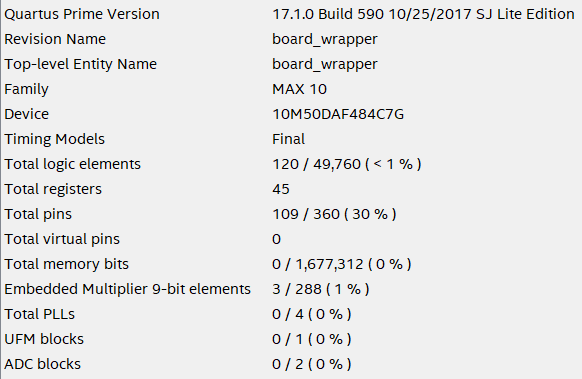
\includegraphics[width=0.8\linewidth]{images/z2_4}
		\caption{}
		\label{fig:z24}
	\end{figure}
	
	\begin{figure}[H]
		\centering
		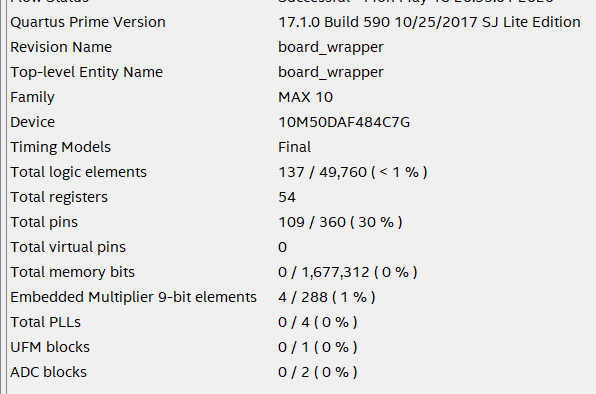
\includegraphics[width=0.8\linewidth]{images/z2_5}
		\caption{}
		\label{fig:z25}
	\end{figure}
	
	\begin{figure}[H]
		\centering
		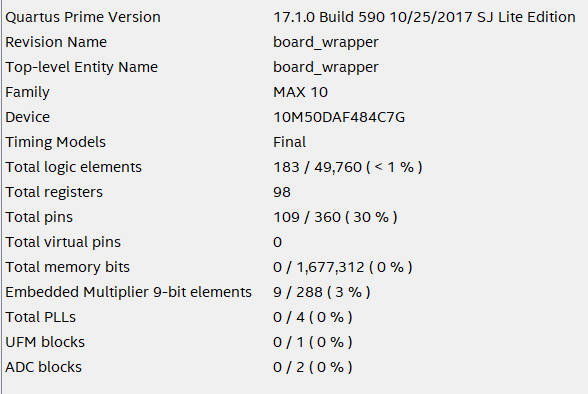
\includegraphics[width=0.8\linewidth]{images/z2_10}
		\caption{}
		\label{fig:z210}
	\end{figure}
	
	
	\subsection{Задание 3}
	
	Выполните имплементацию модуля со значением параметра n = 5, проанализируйте его характеристики и убедитесь, что они не изменились. Убедитесь в работоспособности получившихся реализаций, выполните имплементацию и сравните их	характеристики с характеристиками исходной реализации.
	

	\begin{figure}[H]
		\centering
		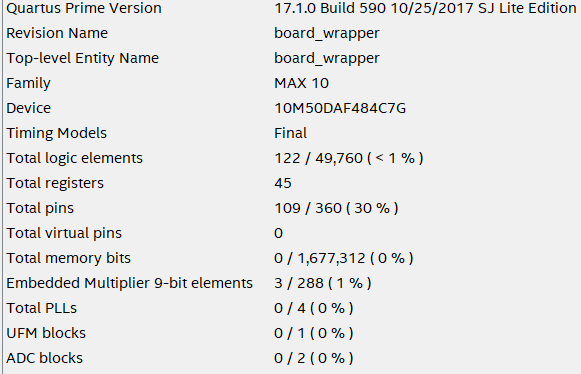
\includegraphics[width=0.8\linewidth]{images/z3_4}
		\caption{}
		\label{fig:z34}
	\end{figure}

	\begin{figure}[H]
		\centering
		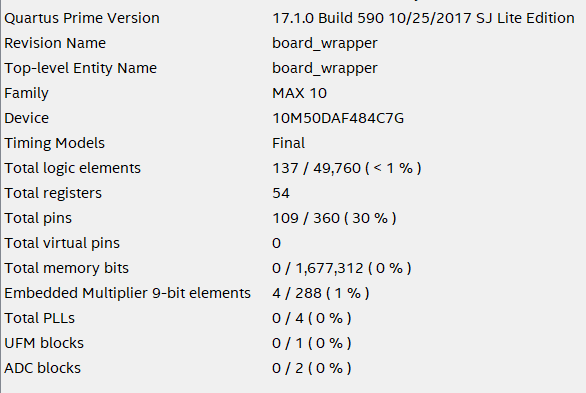
\includegraphics[width=0.8\linewidth]{images/z3_5}
		\caption{}
		\label{fig:z35}
	\end{figure}

	\begin{figure}[H]
		\centering
		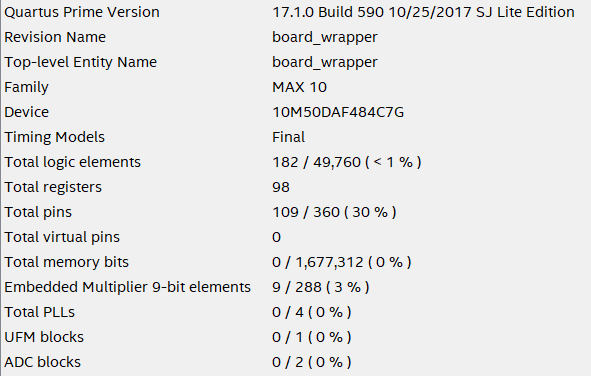
\includegraphics[width=0.8\linewidth]{images/z3_10}
		\caption{}
		\label{fig:z310}
	\end{figure}
	

	\section{Задания для самостоятельной работы}
	
	Квадратный корень
	
	
	
	
	
%%%%%%%%%%%%%%%%%%%%%%%%%%%%%%%%%%%%%%%%%%%%%%%%%
%%%%%%%%%%%%%%%%%%%%%%%%%%%%%%%%%%%%%%%%%%%%%%%%%
%%%%%%%%%%%%%%%%%%%%%%%%%%%%%%%%%%%%%%%%%%%%%%%%%
	\section{Контрольные вопросы}
	
	Подчезерцев Алексей:
	
	\begin{enumerate}
		\item 9. В каких случаях введение сигнала enable в конвейерную схему может отрицательно сказаться на энергопотреблении? 
		
		Динамическое энергопотребление линейно зависит от интенсивности переключения транзисторов.
		Транзисторы переключаются при изменении значения входных сигналов, и эти
		изменения распространяются по схеме даже тогда, когда вычисление само по себе не
		требуется. Поэтому при увеличении тактовой частоты динамическая составляющая
		энергопотребления также увеличивается. Сигнал enable позволяет добавить данные высокопроизводительные блоки в схему.
	
		\item 2. В чем разница между внутренней и внешней фрагментацией в конвейерных схемах?
		Каким образом эти типы фрагментации влияют на эффективность конвейерной	схемы?
		
		Неравенство задержек на стадиях конвейера называется \textbf{внутренней фрагментацией}.
		
		В том случае, если определенный вычислительный ресурс какой-либо стадии не востребован для
		обработки какого-либо типа запросов, поступление такого запроса приведет к простаиванию вычислительного
		ресурса и снижению потенциальной эффективности конвейера. Это простаивание
		называется \textbf{внешней фрагментацией}.
		
		\item 10. Разработчик аппаратного блока получил критическую задержку в 20 нс на одной из стадий конвейера (на каждой стадии запрос обрабатывается один такт). После некоторых размышлений он сделал эту стадию многотактной, что снизило критическую задержку в конвейере до 10 нс. 20 \% запросов на этой стадии стали занимать по четыре такта, а 80 \% запросов занимают один такт. На сколько	изменилась максимальная тактовая частота конвейера и его средняя пропускная способность?
		
		Была частота 50МГц, стала 100МГц.
		
		Средняя пропускная способность $BW_{mean} =  \dfrac{1}{(0.2 * 4 + 0.8 * 1) * 10ns} = 62.5MHz$

	\end{enumerate}
	
	Солодянкин Андрей:

	\begin{enumerate}
		\item 4. При каких свойствах вычислительной нагрузки и стратегии оптимизации применение	конвейерной реализации является предпочтительным по сравнению с многотактной и наоборот?
		
		Сравнение реализаций по аппаратным затратам
		\begin{itemize}
			\item Лучше конвейерная реализация: максимальная частота, интервал инициации (такт), МОп/С, задержка (нс);
			
			\item Лучше многотактовая реализация: Аппаратные ресурсы, энергопотребление;
			
			\item Одинаково: Задержка(такт).
		\end{itemize}
		
		\item 7. Алгоритм состоит из восьми одинаковых последовательно зависимых операций.	Кроме того, результат третьей операции используется в первой операции у следующего запроса. Какова будет структура конвейера, оптимизированного по пропускной способности?
		
		Объединяем каждые 3 операции в один такт, таким образом, После окончания первого такта уже появятся данные для начала работы следующей операции. Внешняя фрагментация минимальна.
	
		\item 5. Необходимо спроектировать аппаратный блок. Существует возможность выбрать один из двух алгоритмов. Первый из них состоит из трех последовательно зависимых операций со следующими задержками: Ll = 20 нс, L2 = 15 нс, LЗ = 15 нс. Второй	алгоритм состоит из двух последовательно зависимых операций со следующими задержками: Ll = 25 нс, L2 = 15 нс. Задержка на буферизацию близка к нулю (ею	можно пренебречь). 
		
		Какой именно из двух алгоритмов и какую именно реализацию (комбинационную или конвейерную) следует выбрать для аппаратного блока? 		
		Какую стратегию оптимизации (по пропускной способности или по задержке) следует выбрать? 		
		Какие характеристики (пропускная способность и задержка) будут у этих блоков?
		
		Для первой реализации подходит конвейерная реализация, с частотой 50МГц, пропускная способность будет также 50 МГц, оптимизация по пропускной способности.
		
		Для второй реализации подходит комбинационная реализация, частота будет 25 МГц, пропускная способность будет также 25 МГц, оптимизация по задержке.
		
		
		
	\end{enumerate}
	
	\section{Выводы по работе}
	
	В ходе работы получен опыт проектирования схем в программе Quartus с помощью языка Verilog.
	Полученное устройство было протестировано с помощью бенчтестов в программе Quartus Simulation Waveform editor.
	В процессе работы были смоделированы устройства для работы с периферийными устройствами.
	В процессе был получен опыт работы с платой DE10-Lite, на которой проверялась работоспособность полученного устройства.
	
	\newpage 
	\renewcommand{\refname}{{\normalsize Список использованных источников}} 
	\centering 
	\begin{thebibliography}{9} 
		\addcontentsline{toc}{section}{\refname} 
		\bibitem{Verilog} Thomas D., Moorby P. The Verilog Hardware Description Language. – Springer Science \& Business Media, 2008.
		\bibitem{citekey} Khor W. Y. et al. Evaluation of FPGA Based QSPI Flash Access Using Partial Reconfiguration //2019 7th International Conference on Smart Computing \& Communications (ICSCC). – IEEE, 2019. – С. 1-5
	\end{thebibliography}
	
\end{document} % конец документа
